\chapter{Conoscenze di Base}
\label{conoscenze}

In questa sezione si introducono i concetti necessari per proseguire con la lettura dei capitoli successivi. 

\section{Crittografia asimmetrica}
\label{asimmetrica}

La crittografia asimmetrica è un tipo di crittografia in cui ogni attore possiede una coppia di chiavi: una \textbf{pubblica} e una \textbf{privata}. Gli usi della crittografia asimmetrica sono due:
\begin{itemize}
	\item Cifrare le comunicazioni: tramite la chiave pubblica del destinatario è possibile cifrare un messaggio che solo il destinatario può decifrare usando la propria chiave privata.
	\item Firmare digitalmente: tramite la propria chiave privata un attore può apporre su un messaggio, autenticandolo, la firma, la quale può essere verificata tramite la chiave pubblica del firmatario.
\end{itemize}

\section{Single Sign-On}
\label{sso}

% AGGIUNGERE ATTORI

Il \emph{Single Sign-On} è un protocollo ampiamente diffuso utilizzato per autenticare utenti a servizi Web. Il protocollo è eseguito da un utente, un User Agent, un Identity Provider e un Service Provider. L'User Agent è un software usato dall'utente che permette l'interazione con un contenuto Web. L'Identity Provider è un attore terzo che si occupa di fornire un sistema di autenticazione sicuro, creando e gestendo le credenziali degli utenti, a servizi Web che lo richiedano. L'Identity Provider possiede molteplici Identity Server presso cui gli utenti devono eseguire le operazioni di autenticazione. Il Service Provider è un fornitore di servizio Web che non implementa sistemi di autenticazione propri, ma si avvale di quelli messi a disposizione dall'Identity Provider. Qualora l'utente si autentichi con successo presso l'Identity Server, gli viene fornito un token di autenticazione firmato dell'Identity Server, che deve presentare al Service Provider per poter fruire di quel servizio.  Una volta presentato il token al Service Provider, l'utente risulta autenticato a tutti quei servizi messi a disposizione dal Service Provider che fanno uso dello stesso Identity Provider. Da qui l'accezione \emph{single} di \emph{sign-on}.

\section{Survivability}
\label{surviv}

La centralizzazione dello schema SSO lascia spazio ad attacchi in cui un malintenzionato prenda il controllo dell'Identity Server e utilizzi la chiave privata dello stesso per firmare token di autenticazione forgiati arbitrariamente, così da poter poi impersonare qualunque utente egli voglia. Giungono in aiuto gli schemi cosiddetti \emph{survivable SSO} che possono limitare tali criticità sfruttando più Identity Server. Un singolo Identity Provider gestisce pertanto più Identity Server e l'utente deve autenticarsi presso un sottoinsieme di questi, i quali rilasciano un \textbf{token} firmato collettivamente. 

La componente \emph{survivable} risiede nel fatto che si tollera un certo numero di Identity Server violati e, di conseguenza, si richiede un token in funzione di questo numero. Con una soglia di tolleranza di server maligni sufficiente si riesce a garantire l'integrità del meccanismo di autenticazione e un overhead dovuto alla reiterazione dei passaggi trascurabile.

\section{Passwordless}
\label{passwordless}

L'autenticazione passwordless è un metodo di autenticazione che permette all'utente di effettuare il login ad un servizio senza la necessità di conoscere una password o più genericamente senza una conoscenza considerata segreta. Tipicamente utilizza una coppia di chiavi crittografiche, una privata e una pubblica: la prima è generata e immagazzinata sul dispositivo dell'utente, mentre la seconda è inviata al server così che esso possa verificare l'autenticità dei messaggi ricevuti. La chiave privata, o segreta, non lascia mai il dispositivo su cui è stata creata e per accedervi è necessaria l'autorizzazione ottenuta tramite \textbf{mediazione} da parte dell'utente. Un'azione è detta mediata da un utente qualora sia necessario il suo esplicito consenso, il quale può avvenire, ad esempio, premendo il bottone sul dispositivo fisico.

La registrazione passwordless e, conseguentemente, l'autenticazione sono svolte seguendo un meccanismo \emph{challenge-response}: al pervenire di una richiesta di registrazione il server invia una cosiddetta \emph{challenge}. L'utente che ha iniziato l'operazione ha il compito di apporre, tramite propria chiave privata, una firma crittografica sulla challenge e di fornire in risposta al server la challenge firmata accompagnata dalla chiave pubblica. In questo modo il server verifica l'autenticità della firma tramite la chiave appena ricevuta e in caso di esito positivo immagazzina la chiave pubblica. La fase di autenticazione è svolta in modo analogo, se non che il server è già in possesso della chiave pubblica e non è quindi necessario inviarla.

Ne deriva che non viene scambiato alcun segreto e l'unica interazione richiesta all'utente è quella in fase di firma della challenge. Anche durante la stessa l'utilizzatore non deve inserire codici o password, ma semplicemente mediare l'operazione tramite uno dei metodi sopra elencati. Sfruttando l'autenticazione passwordless è possibile sopperire alle criticità tipiche dei segreti a bassa entropia come le password, quali phishing, brute forcing etc. 

\section{FIDO}
\label{fido}

FIDO Alliance è un'associazione nata nel 2013 con lo scopo di migliorare i sistemi di autenticazione tramite la diffusione dell'autenticazione passwordless. Sono gli autori di \emph{FIDO}, un set di specifiche che include gli standard \textbf{CTAP} e \textbf{WebAuthn}. Nel corso degli anni vi è stato un susseguirsi di iterazioni dello standard: dapprima noto come Universal Authentication Factor, divenne poi Universal 2nd Factor per giungere infine alla versione corrente FIDO 2.0. 

Il protocollo CTAP definisce le API che un client può utilizzare per comunicare con un autenticatore. Il protocollo WebAuthn definisce invece le API per l'autenticazione a servizi web sfruttando le chiavi crittografiche. 

In particolare, questi protocolli definiscono tutto il necessario per programmare un autenticatore e un server come: strutture dati, metodi, requisiti di funzionamento, encoding dei dati etc.

\subsection{Rilevamento tentativi di clonazione}
\label{fido:clonazione}

Compito dell'Identity Server è anche quello di rilevare eventuali tentativi di duplicazione dell'autenticatore fisico. Per fare ciò lo standard FIDO prevede un \textbf{contatore}, sia esso globale o multiplo, aggiornato dall'autenticatore ad ogni operazione avvenuta con successo. Il contatore prende il nome di \emph{signature counter}. Il server mantiene in memoria l'ultimo valore ricevuto e, all'interazione successiva, controlla che non vi siano discrepanze. Ad esempio, ipotizzando di avere allo stesso tempo:
\begin{itemize}
	\item Un autenticatore originale con contatore pari a \emph{m}
	\item Un autenticatore clone dell'originale con contatore pari a \emph{m}
\end{itemize}
Se l'autenticatore originale si autentica presso un servizio, questi aggiorna il proprio contatore a ${m+1}$. Il clone, tentando di autenticarsi allo stesso servizio, fornisce un valore del contatore pari a \emph{m}, dunque minore di quello salvato in memoria dal server al momento dell'ultima interazione con l'autenticatore originale. In questo modo, il server riconosce il clone in quanto tale. 

Ne consegue che il rilevamento del tentativo di clonazioni basato sul contatore risulta:
\begin{itemize}
	\item Inefficace finché il clone non procede ad autenticarsi
	\item Fallace se il clone procede ad autenticarsi prima dell'originale: quest'ultimo viene di fatto invalidato nonostante sia legittimo
\end{itemize} 

\begin{center}
	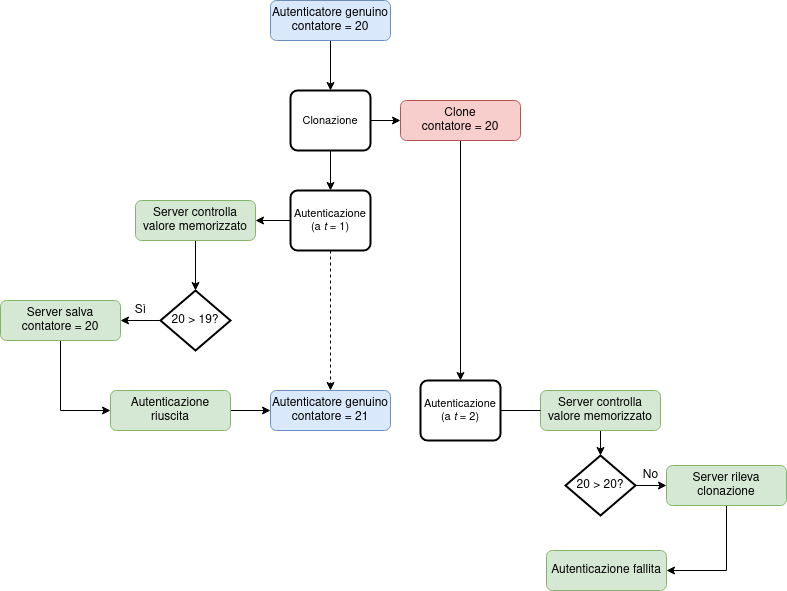
\includegraphics[width=1.1\columnwidth]{figures/test}
	\label{fig:flowchart_contatore}
\end{center}